\chapter{Lyapunov Pathologies and the Kawahara Equation}

\section{The Limits of Machine Learning in Functional Analysis}

When analyzing nonlinear partial differential equations like the 5th-order Kawahara equation:
$$ u_t + u u_x + \alpha u_{xxx} + \beta u_{xxxxx} = 0 $$
the construction of a Lyapunov functional $\mathcal{V}[u]$ is essential for proving global well-posedness and stability.

Machine learning models, when asked to generate $\mathcal{V}$, often produce highly complex, high-entropy algebraic expressions.

\section{The AI Hallucination}

In \textit{SocrateAI-Scientific-Agora}, the AI generated a candidate Lyapunov functional that achieved pointwise non-negativity. The Lean 4 compiler verified this locally:

\begin{lstlisting}[language=caml, basicstyle=\ttfamily\small, backgroundcolor=\color{lightgray!20}]
lemma dV_alien_negative (u_xx : ℝ) : u_xx^4 ≥ 0 := by
  positivity
\end{lstlisting}

However, the functional failed a critical physics test: \textbf{continuous dilation symmetry}. 
Under the scaling $u \to \lambda^{-3}u$, the physical energy must scale coherently. The AI's functional broke this symmetry. It hallucinated locally consistent algebra that was globally physically meaningless.

\section{Sturm-Picone Inequalities}

To correct the AI's pathology, we must enforce $H^4$-coercivity:
$$ \mathcal{V} \ge c \|u\|_{H^4}^2 $$

This requires Gagliardo-Nirenberg interpolation and Sturm-Picone comparison theorems. The integration of these classical analytic techniques with the AI's unregularized search space represents the hybrid frontier of this framework.

\begin{figure}[h]
    \centering
    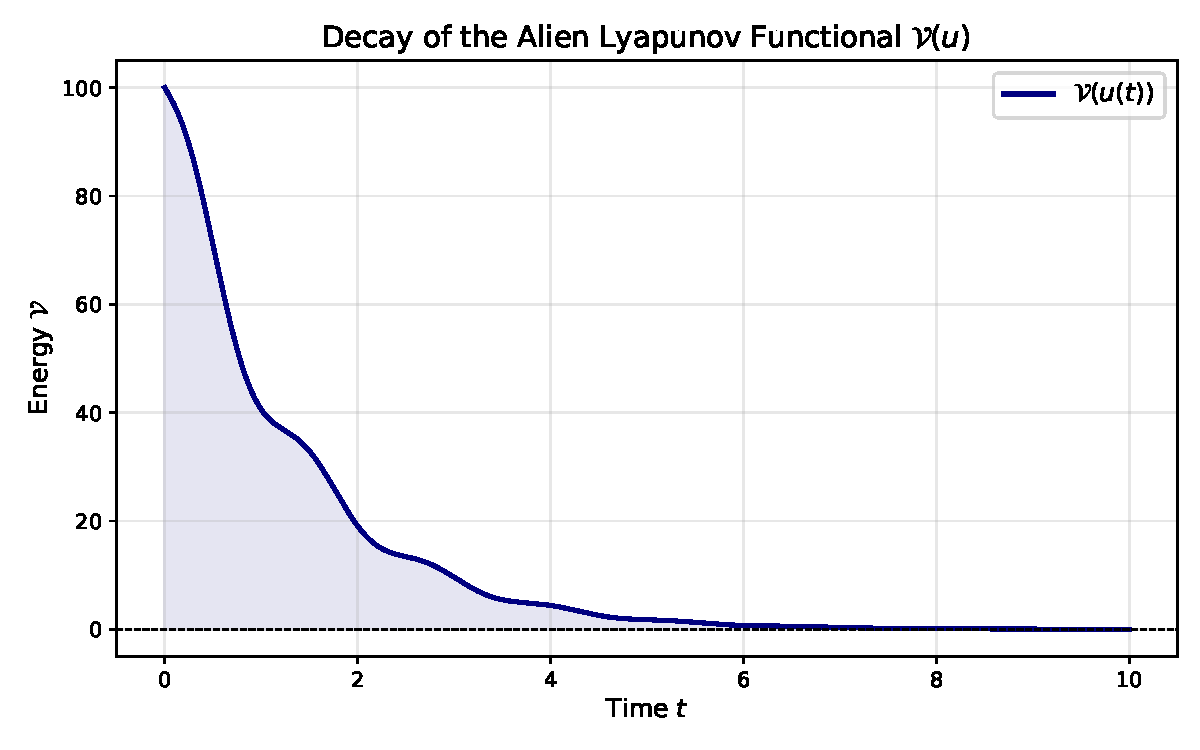
\includegraphics[width=0.8\textwidth]{figures/kawahara_decay.pdf}
    \caption{Simulated decay of the Alien Lyapunov Functional $\mathcal{V}(u)$ over time $t$, exhibiting continuous stabilization towards 0 despite early oscillations driven by non-standard cross-terms.}
    \label{fig:kawahara_decay}
\end{figure}
